\chapter{Status of Ceramic Breeder Modeling and Analysis}\label{sec:modeling-state}
A common problem plaguing the study of packed beds is the disconnect between the scale of physics influencing the behavior of the packed bed and the scale of quantifiable and measurable physics in experiments. In the laboratory we are limited to measurements such as the stress and strain of the entire packed bed and then are left to infer how the internal packing of the ensemble leads to the measurable values. Unfortunately, the stress-strain response of a packed bed is often not unique to a specific `state' such as one might use to describe an ideal gas. Nevertheless, considerable work has been done by experimenters at characterizing properties of a wide range of pebbles types and materials.

% The solid breeder in many current designs feature sub-module units of packed beds. From the point of view of pebble bed thermo-mechanical properties, this has the advantage of producing units individually that can be tested and qualified to desired packing states (and therefore thermo-mechanics) during the design phase. 

% The thermophysical and thermo-mechanical properties of pebble beds have been studied extensively [cite many of the experimental papers]. From experimental measurements, and the assumption that a pebble bed can be treated as a continuous media, researchers have developed phenomenological formulas relating properties of pebble bed to other, measurable, macroscopic properties [cite many of the modeling papers]. For instance, an effective thermal conductivity can be given for the packed bed given a certain gas and stress on the bed. These effective material properties are useful for the design and qualification of tritium breeding modules. But it must be understood that the material properties of a pebble bed are a function of their history and will evolve in time as the morphological features of the pebble bed likewise evolve in time. Therefore there is a need to predict the morphological changes to the pebble bed and the subsequent impact on the bed's thermophysical properties so that solid breeder designers may have reliable temperature control of the pebble bed over the duration of the use of the breeder in the reactor. 


% Ceramic breeders, by their nature, are brittle and prone to cracking under external mechanical loadings. These breeders, in the form of packed beds of pebbles, are loaded into a box-like structure for tritium fuel production in a fusion reactor. When subjected to nuclear heating in a reactor, a strong mechanical loading arises from the differential thermal expansion between breeder pebbles and their containing structure. 

In \cref{sec:blanket-design}, we described how thermally-induced stress arises in the ceramic breeder volume. Research efforts have therefore been aimed at developing a thorough understanding and characterization of the thermo-mechanics of ceramic breeder pebble beds. Such an understanding is essential to providing confidence in the performance and lifetime of a ceramic breeder blanket design. In particular, a significant effort of the pebble bed thermo-mechanics study is on the development of modeling simulation tools. We will describe, in brief, some of the major experimental findings as they relate to the modeling efforts for ceramic pebble beds.

Reimann\etal~have conducted an extensive experimental study of the stress-strain relations of the ceramic breeder pebble beds using an oedometric test apparatus \cite{Piazza2002811,Reimann:2002kl,Reimann:2003qc,Reimann:2002mi,Reimann:2001il}. The most significant macroscopic experimental phenomena witnessed in the pebble bed are an irreversible plastic strain when the load is removed, a non-linear elasticity, a pressure-dependent plasticity, and a volumetric creep.  A particularly noticeable feature, clearly demonstrated in Fig.~\ref{fig:mti}, is the reduced amount of irreversible strain when subjected to additional loading cycles after the first unloading. This may suggest the existence of a semi-equilibrium packing state in the pebble bed which can be reached after applying a pre-load to account for the large strain in the first cycle of a pebble bed. This semi-equilibrium packing state is a feature which may be advantageous for use in a fusion reactor.

Zhang\etal~ran similar cyclic pressure experiments to illuminate the existence of more steady stress-strain responses of packed beds under different pressures. 

To study the temperature effect in Reimann's studies, the bed is freely heated to the desired working temperature before the pressure load is applied. Under the same loading condition, the bed behaves much softer at higher temperatures. The bed stiffens as the pressure increases. An illustration of this phenomenon is presented in Fig.~\ref{fig:UCT} for a lithium orthosilicate pebble bed between $50-850^\circ$C. At higher temperatures (such as $> 650^\circ$C), a creep-like behavior becomes apparent. The creep behavior allows the pebble bed to relax and sustain higher stresses, however one needs to avoid sintering. The data was used to correlate creep rate as a function of temperature, stress, and time for both lithium orthosilicate, lithium metatitanate, and beryllium pebble beds \cite{Buhler:2002qf,Reimann:2001il,Reimann:2005qa}.


\begin{figure}[t!]
	\begin{center}
	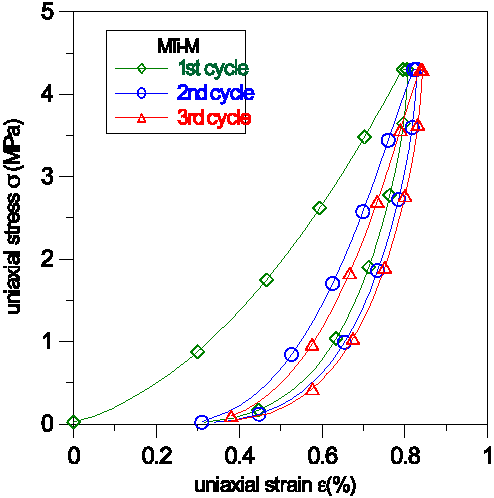
\includegraphics[width=0.4\textwidth]{chapters/figures/Fig-1}
	\caption{Example of uniaxial compression testing results for lithium metatitanate pebble bed \cite{vanderlaan2011}.}
	\label{fig:mti}
	\end{center}
\end{figure}

\begin{figure}[t!]
	\begin{center}
	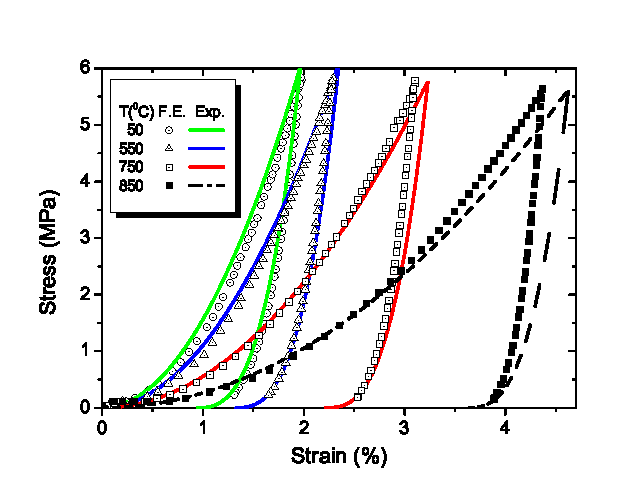
\includegraphics[width=0.5\textwidth]{chapters/figures/Fig-2}
	\caption{Example of uniaxial compression testing results compared with predictions from material constitutive equations for lithium orthosilicate pebble beds at different temperatures \cite{Gan:2008kx}.}
	\label{fig:UCT}
	\end{center}
\end{figure}


% Thus for packed beds of ceramics for tritium breeding, phenomenological models have been developed based on empirical observations from the controlled environment of laboratory experiments. 
When we consider the pebble bed from the standpoint of engineering continuum mechanics, packed beds cannot be adequately described by traditional models of either solids or liquids alone. Under compression, a packed bed responds like a solid with non-linear elasticity and a plasticity that is history-dependent. At the same time, the packed bed can obviously not support any tensile pressure and will often behave as an extremely viscous liquid as it may fill in voids under just the force of gravity. Nevertheless, phenomenological models, derived from the volumes of collected data, have been developed, using effective material properties for the ceramic pebble bed, that describe the pebble beds in an Eulerian manner that provide reliable information on the initial states of breeder volumes in the fusion reactor environment and allow reasonable design predictions of the thermo-mechanics of the breeding blanket. 

In spite of the shortcomings of a continuum approach, it is the only option which currently allows treatment of the pebble beds with standard finite element modeling (FEM) that can be scaled up to the breeder system. To employ FEM, mathematical models written in terms of average quantities and containing effective parameters are used. These models deduce a set of constitutive equations to be implemented in the framework of a finite element code.  There are two major variants of phenomenological modeling approaches developed among institutions, including: (1) A non-linear elastic model and a modified Drucker-Prager-Cap theory for plastic strain \cite{Gan2007189,fokkens2003}; and (2) A hyper-porous non-linear elastic model and a Gurson model for the plastic model \cite{DellOrco:2007hc,DellOrco:2010zr,DiMaio20081287}. Another approach was taken by Ref.\cite{fokkens2003} wherein the authors employed two different elasticity laws for the loading and unloading branches. Alongside the development of the modeling techniques, several large scale pebble bed thermo-mechanics experiments were conducted. These experiments were intended to reveal the underlined thermo-mechanical characteristics of ceramic breeder pebble beds, and provide data for benchmarking the developed models. The vast amount of work done on modeling the pebble beds in the FEM framework can be found in literature. \cite{DellOrco:2007hc,DellOrco:2010zr,DiMaio20101234,Gan2007189,Gan2007189,Gan:2009vn,Gan:2010lh,Gan:2010kc,DellOrco:2007hc,DellOrco:2010zr,DiMaio20101234,Gan2007189,DellOrco:2007hc,DiMaio20101234} A study was also published in 2012 that summarized, compared, and highlighted features of the models under development at the time.\cite{ying2011isfnt}

We will devote the rest of this chapter to the discussion of advances of an alternative modeling approach for solid breeder analysis. In this modeling strategy, we consider the pebble bed as a system of distinct interacting bodies that are subject to fundamental forces which result in independent motions. This modeling approach, called the discrete element method (DEM), is the framework upon which the work of this dissertation is laid, as such we will go into more detail on the history of DEM's use in fusion science and technology research.

\section{DEM for Tritium Breeders}

A thorough review of the physics behind DEM will be given in \cref{sec:dem-studies}. For now, we will simply discuss some major results of the implementation of DEM in solid breeder research.

The Discrete Element Method (DEM) introduced by~\cite{Cundall1979} has been shown to be a promising tool to study the behavior of granular systems through the interaction between the individual particles. DEM was first applied to study the micro-mechanical aspects of cyclic thermal loads on the relaxation of stress in pebble beds for fusion reactors.\cite{Lu2000b,Ying2002}. An iterative relaxation strategy of DEM was used to study the internal contact forces in a pebble bed under an external load by An\etal\cite{An20072233} The same DEM tools, and the insight provided by which, were also used to initiate DEM-based investigations of creep between pebbles under thermal and mechanical loads.\cite{An20071393} While An\etal~studied the pebble assemblies in rectangular and cylindrical containers bounded by a elastic walls, computational requirements prevented more than a few thousand particles in the ensemble with rigid walls.\cite{An20072233} Following An's work, the DEM torch was passed across the pond to researchers at KIT where they began to improve upon the initial studies begun at UCLA.

\begin{figure}[!ht]
	\centering
	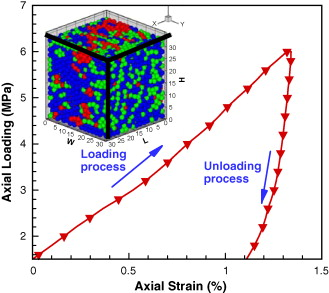
\includegraphics[width=0.5\textwidth]{chapters/figures/1-s2.0-S092037960700049X-gr1.jpg}
	\caption{Stress–strain behaviors of granular materials in a rectangular box under uni-axial compaction from DEM are qualitatively matched to behaviors seen experimentally.}
\label{fig:an-uniaxial-compression}
\end{figure}

The effect of packing factor, geometry of the assembly on the overall stress-strain response under uni-axial compression tests (UCT) has been thoroughly investigated.\cite{Gan:2010uq} Gan\etal~pebble assemblies in a cubic box with periodic boundary conditions to prevent the influence of boundaries dominating the ensemble response to loads.\cite{Gilabert2007} In the DEM uni-axial compression studies (see Fig.~\ref{fig:an-uniaxial-compression}), a non-linear stress-strain response and a characteristic residual strain after unloading (analogous to plastic strain in continuum systems) is observed akin to the experimental results.\cite{Reimann:2000tw} It was shown that the average coordination number, average normal contact force and the maximum normal contact force in the assembly has a unique functional relation (nonlinear, linear and linear, respectively) with the hydrostatic pressure or the applied pressure independent of the packing factor.\cite{Gan:2010uq,An20071393} These functional relations may be used as master curves for the micro-macro correspondence in the pebble bed thermo-mechanics studies.

Recently, the effect of the pebble size distribution on the overall thermo-mechanical behavior of the pebble assembly is studied by Annabattula\etal\cite{Annabattula2011}. They consider the pebble size distribution of ceramic breeder pebbles (\lis) with a diameter range of $0.25\ \mathrm{mm}$-$0.65\ \mathrm{mm}$. Figure~\ref{fig:pebble-assembly-potential-energy} shows a binary pebble assembly in a periodic box. The colors indicate stored elastic strain energy of the pebble (red: maximum and blue: zero). The assembly has a maximum pebble radius $\rmax=0.25$ mm with the pebble size ratio $\rstar=\rmin/\rmax=0.6$, relative volume fraction $\vstar=\vmax/V=0.7$ and a packing factor $\eta=0.643$. The average stress in a granular assembly can be deduced from the contact forces between individual grains.

\begin{figure}[!ht]
	\begin{center}
	\begin{minipage}{0.45\textwidth}
	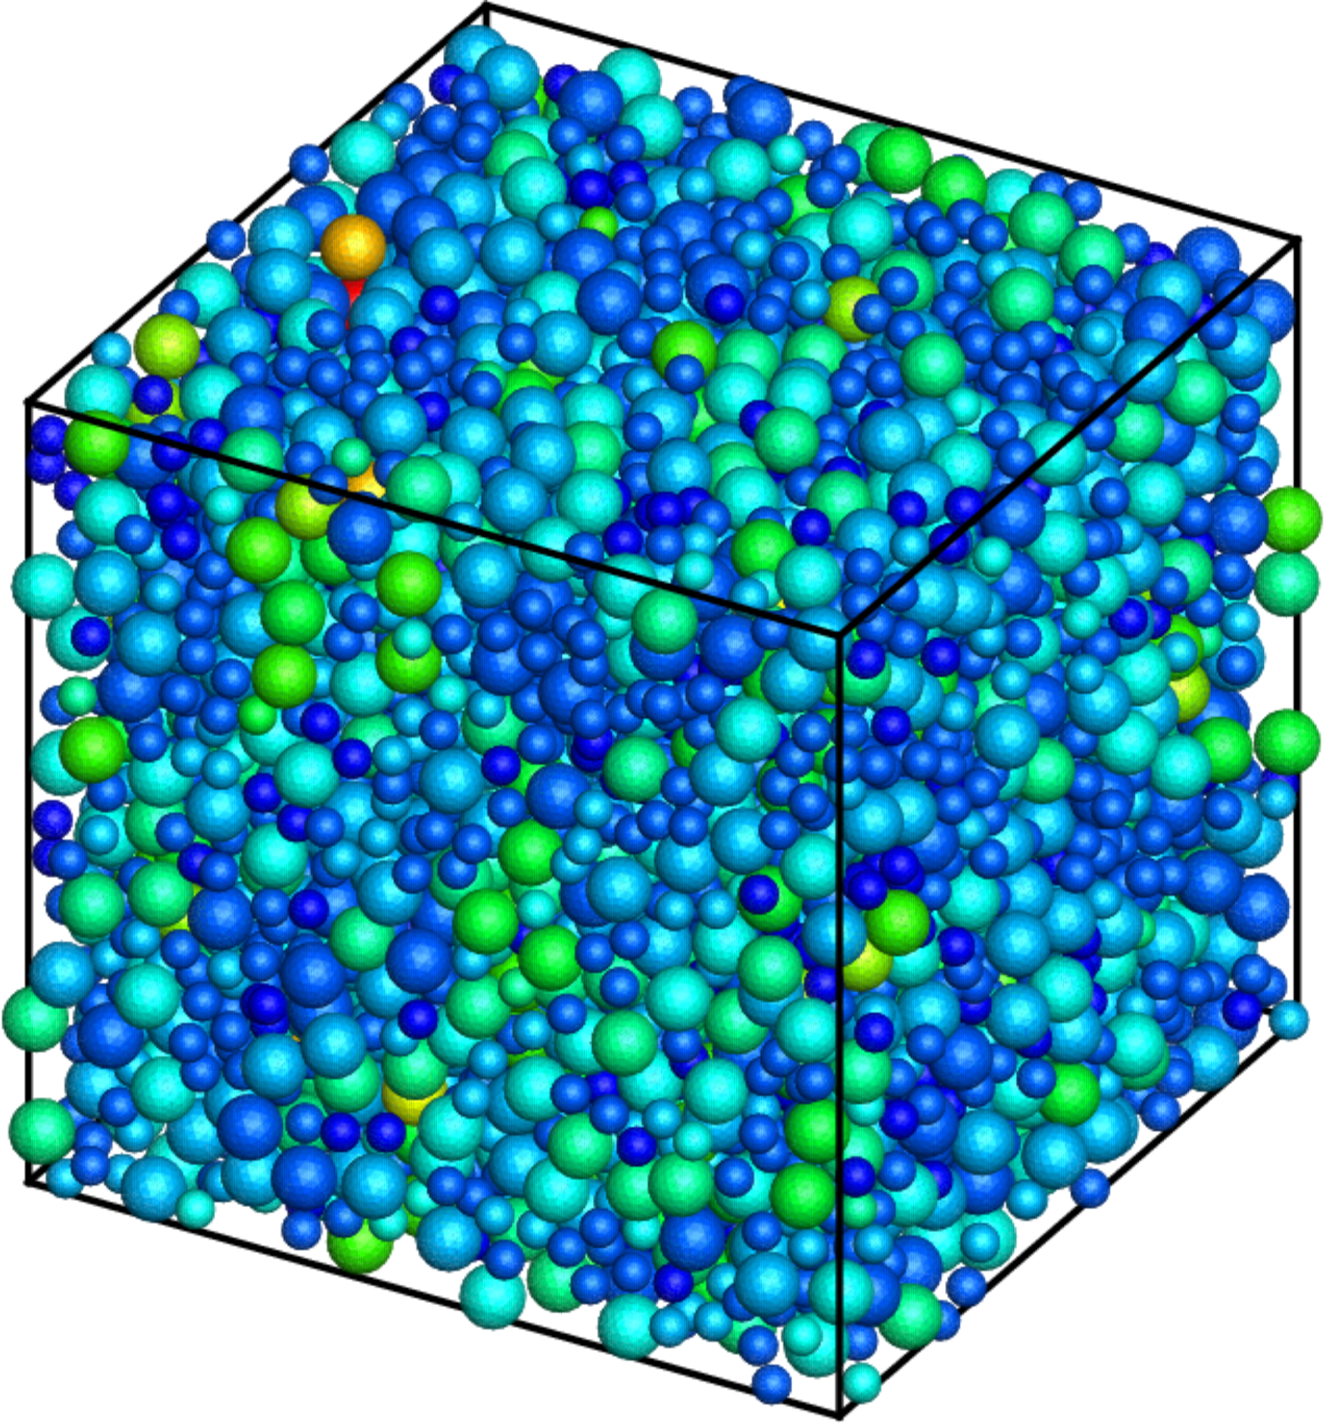
\includegraphics[width=6cm]{chapters/figures/Fig-3}
	\begin{picture}(15,15)(340,-120)
	\put(330,-80){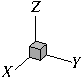
\includegraphics[scale=1]{chapters/figures/Fig-3b}}
	\end{picture}
	\end{minipage}
	\end{center}
	\caption{A binary pebble assembly with $\rstar = 0.6$ and $\vstar=0.7$ showing the stored elastic energy of the pebbles at $\epsilon_{33}=1.5\%$; pebbles of radius $r_s$ (small) and $r_g$ (large).}
	\label{fig:pebble-assembly-potential-energy}
\end{figure}

Another aspect of interest in the study of mechanics of pebble beds is the crush behavior of individual pebbles and their impact on the over all pebble bed response. DEM was used to study the behavior of a crushable pebble assembly with the crush load data for \lis pebbles (for individual pebbles) measured at KIT for pebbles of diameter 0.5 mm. 

A probabilistic method for analyzing the crush events of individual pebbles and a procedure with the combination of DEM and experimental data to obtain crush load probability has been reported by~\cite{Gan:2010kc}. Figure~\ref{fig:cdf_pebbles} shows the cumulative distribution function as a function of the hydrostatic pressure placed on the bed. The probability analysis, derived from DEM calculations, provides quantitative report of pebble crushing as a function of a specific hydrostatic pressure. The results of this analysis exemplify the growing strength of DEM techniques for analyses connecting global pebble bed loads to individual pebbles.

\begin{figure}[!ht]
  \begin{center}
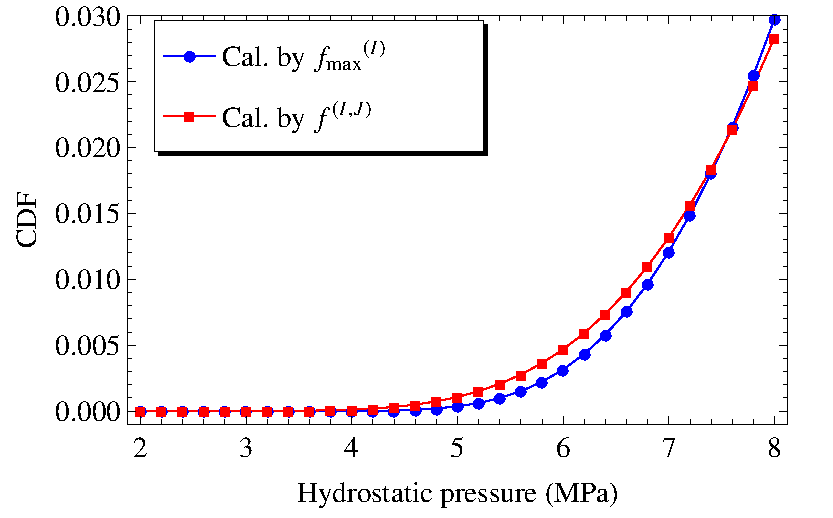
\includegraphics[width=0.5\textwidth]{chapters/figures/Fig-4}
\end{center}
 \caption{Cumulative distribution functions for crushing of individual pebbles inside the bed for as-fabricated pebbles, calculated by (1) maximum contact forces and (2) all inter-particle contact forces~\cite{Gan:2010kc}.}
 \label{fig:cdf_pebbles}
\end{figure}

However, it has been shown~\cite{Zhao2010,Zhao2011} that a criterion based on critical stored elastic energy is the most suitable criterion for describing the \lis pebble failure. Hence, the crush load data (provided by fusion materials laboratory at KIT) has been transformed into equivalent elastic strain energy showing a Weibull distribution~\cite{Zhao2010}. This critical energy (randomly generated distribution) is used as the criterion for failure of pebbles in the DEM simulations. First, the assembly is loaded up to 3\% strain in uniaxial compression and then unloaded to a stress-free state. The elastic modulus of the pebble is reduced (from initial value to a small value of 1 kPa) with increase in elastic strain energy of the pebble according to a phenomenological damage accumulation law~cite{Annabattula2011b}. The damage state is frozen at the end of loading step and hence there will be no further damage accumulation in the unloading step. 

Figure.~\ref{fig:stress-strain-effect} shows the results for two types of damage law each with three different realizations. Each realization corresponds to a different random distribution of critical energies assigned to the pebbles in the assembly. The results do not show appreciable sensitivity to random distribution of energies. In the case of gradual damage law, the reduction of the elastic modulus of the pebble starts when the stored elastic energy reaches 50\% of the critical energy for that pebble and the elastic modulus reaches exponentially to its minimum value when the stored elastic energy reaches the critical energy prescribed. In the case of sudden damage this reduction starts at a much later stage when the stored elastic energy reaches 95\% of the critical energy of the pebble. Clearly, the assembly with a sudden damage accumulation shows a higher maximum strength compared to the gradual damage. In the case of the gradual damage, the pebbles start to degrade much earlier (at small strain) than in the case of sudden damage. Hence the critical number of pebbles to fail for the onset of maximum strength is reached earlier (at small strain) in gradual damage. It turns out that a mere 0.2\% pebbles is the critical number for the onset of maximum strength (stress plateau) observed.

\begin{figure}[!ht]
\begin{center}
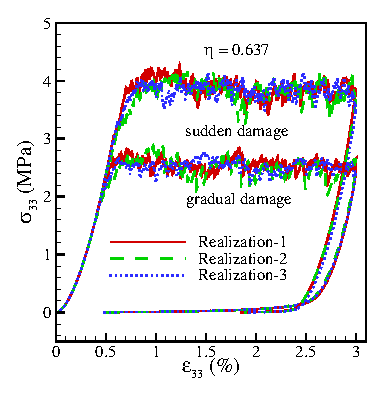
\includegraphics[width=0.4\textwidth]{chapters/figures/Fig-5}
\end{center}
\caption{Stress-Strain response of a granular assembly under uni-axial compression for two different damage evolution laws (gradual and sudden). Each damage evolution criterion is simulated with three different realizations of randomly prescribed critical failure energy for individual pebbles following Weibull distribution.}
\label{fig:stress-strain-effect}
\end{figure}

The nature of damage evolution influences the maximum strength and strain at which the maximum strength is attained while the critical number of failed pebbles for this saturation is independent of the damage evolution law (also see~\cite{Zhao2010}). Also note that the high frequency oscillations during loading in the stress-plateau region represent the failure of new pebbles. The current analysis also shows a creep-like behavior of the stress-strain response and hence the stress-plateaus observed in the experiments~\cite{Reimann:2000tw} may indicate the presence of pebble crushing in addition to the thermal creep mechanism. Furthermore, the residual strain after unloading is large for the system with sudden damage than the system with gradual damage. It should be noted that the assembly with gradual damage has more number of damaged pebbles at the end of loading (at 3\% strain) making the assembly more compliant than in the case of sudden damage. 


%%%%%%%%%%%%%%%%%%%










\section{Experimental Pebble Bed thermo-mechanics Studies}
\subsection{Out-of-pile experiments}
The constitutive equations developed for finite element models were derived from the uniaxial compression experiments, which are not fully representative of fusion operating conditions. A more prototypical experiment should subject a pebble bed to isostatic loading. This could be generated by either an in-pile pebble bed experiment or by making use of differential thermal expansion between a pebble bed and its containing structure. The latter has been attempted with several out-of-pile experiments launched by the HE-FUS 3 facility at ENEA Brasimone. The experiments investigated the thermo-mechanical behavior of pebble beds within geometry much more representative of current breeder designs. These include the medium-scale mock-up exercises of HELICA (HE-FUS3 Lithium Cassette) and HEXCALIBER (HE-FUS3 Experimental Cassette of Lithium Beryllium Pebble Beds) \cite{dellorco:2006,DiMaio20081287}. For those experiments, the pebble layers are heated by electric heaters, and temperature and displacement were measured.

\subsubsection{FZK Benchmarking}
FZK has performed validation of their FEM code against the data collected from the HELICA experiment \cite{Gan:2008kx}. They have also reported the results of simulations of HEXCALIBER but have, as yet, not directly validated against the collected experimental data \cite{Gan:2009vn}.

In the HELICA experiment, the pebble beds experienced six thermal ramps, each applied for an hour, and then the pebble beds were actively cooled with a helium flow. After cooling, the pebble beds were subjected to the another thermal ramp and the process was repeated. DIN reports\cite{dellorco:2006} that the pebble bed temperatures exhibited cyclical behavior. FZK simulated two cycles of the HELICA test and an example of the calculated results and experimental data are shown in Fig.~\ref{fig:FZK_HELICAa} and Fig.~\ref{fig:FZK_HELICAb}. In Fig.~\ref{fig:FZK_HELICAa} we see temperature histories at a particular location (100 mm from the first wall) during a loading-unloading cycle. The simulation results follow the temperature increase during the thermal ramps up until the seventh hour, then again follow the experimental data as the test rig is cooled with the helium coolant. Even with the two-dimensional simplification of the model, there is excellent agreement between calculations and measurements. In Fig.~\ref{fig:FZK_HELICAb} the displacement calculated by FZK is also in strong agreement with the average of measured displacements for the entire duration of the heating-cooling cycle. Because of the overwhelming amount of computer time necessary for the FZK model to complete a fully three-dimensional and transient simulation, the FZK computations of HELICA and HEXCALIBER are carried out in two dimensions; the helium temperature is chosen at an average value of measured inlet and outlet temperatures.

From FZK's numeric simulation arise several important observations: (i) a three-dimensional analysis would provide more detail, spatial temperature variation of e.g. coolants would likely explain much of the deviation between temperature profiles predicted by the simulation and measured in the HELICA experiment; (ii) gap formations, with sizes on the order of a pebble diameter, were detected at the interface of the first wall in ceramic beds; (iii) the maximum hydrostatic pressures seen in the ceramic bed are anticipated to be above the fracturing limit of the lithium ceramic. The consequences of some of these observations, if true and real, are severe enough that they merit careful attention. Gap formation and pebble failure (crush or fracturing) are important topics that must be considered in validation with future experiments.

\subsubsection{DIN Benchmarking}
Because of the characteristics of the DIN model, full three-dimensional simulations were capable of being relatively easily performed. In the framework of benchmarking efforts, DIN has performed validation of their model against experimental results of HELICA, shown in Fig.~\ref{fig:DIN_HELICA} as well as HEXCALIBER, shown in Fig.~\ref{fig:DIN_HEX}.

The results of the DIN model show also strong agreement to the experimental results of HELICA as demonstrated in one example of temperature histories shown in Fig.~\ref{fig:DIN_HELICA}. In this profile, the same location as that modeled by FZK (100 mm from the first wall) is simulated by DIN. The FEM simulations from DIN (Fig.~\ref{fig:DIN_HELICA}) are reported over the six-hour heating portion of a single heating ramp cycle of HELICA. When comparing the results from DIN with those of FZK (in Fig.~\ref{fig:FZK_HELICAa} and Fig.~\ref{fig:FZK_HELICAb}) we see the DIN model has slightly better predictive capabilities for the temperature histories. This may be due attributed to the three-dimensional variations in coolant temperature being captured by the DIN model. 


\begin{figure}[t!]
\centering
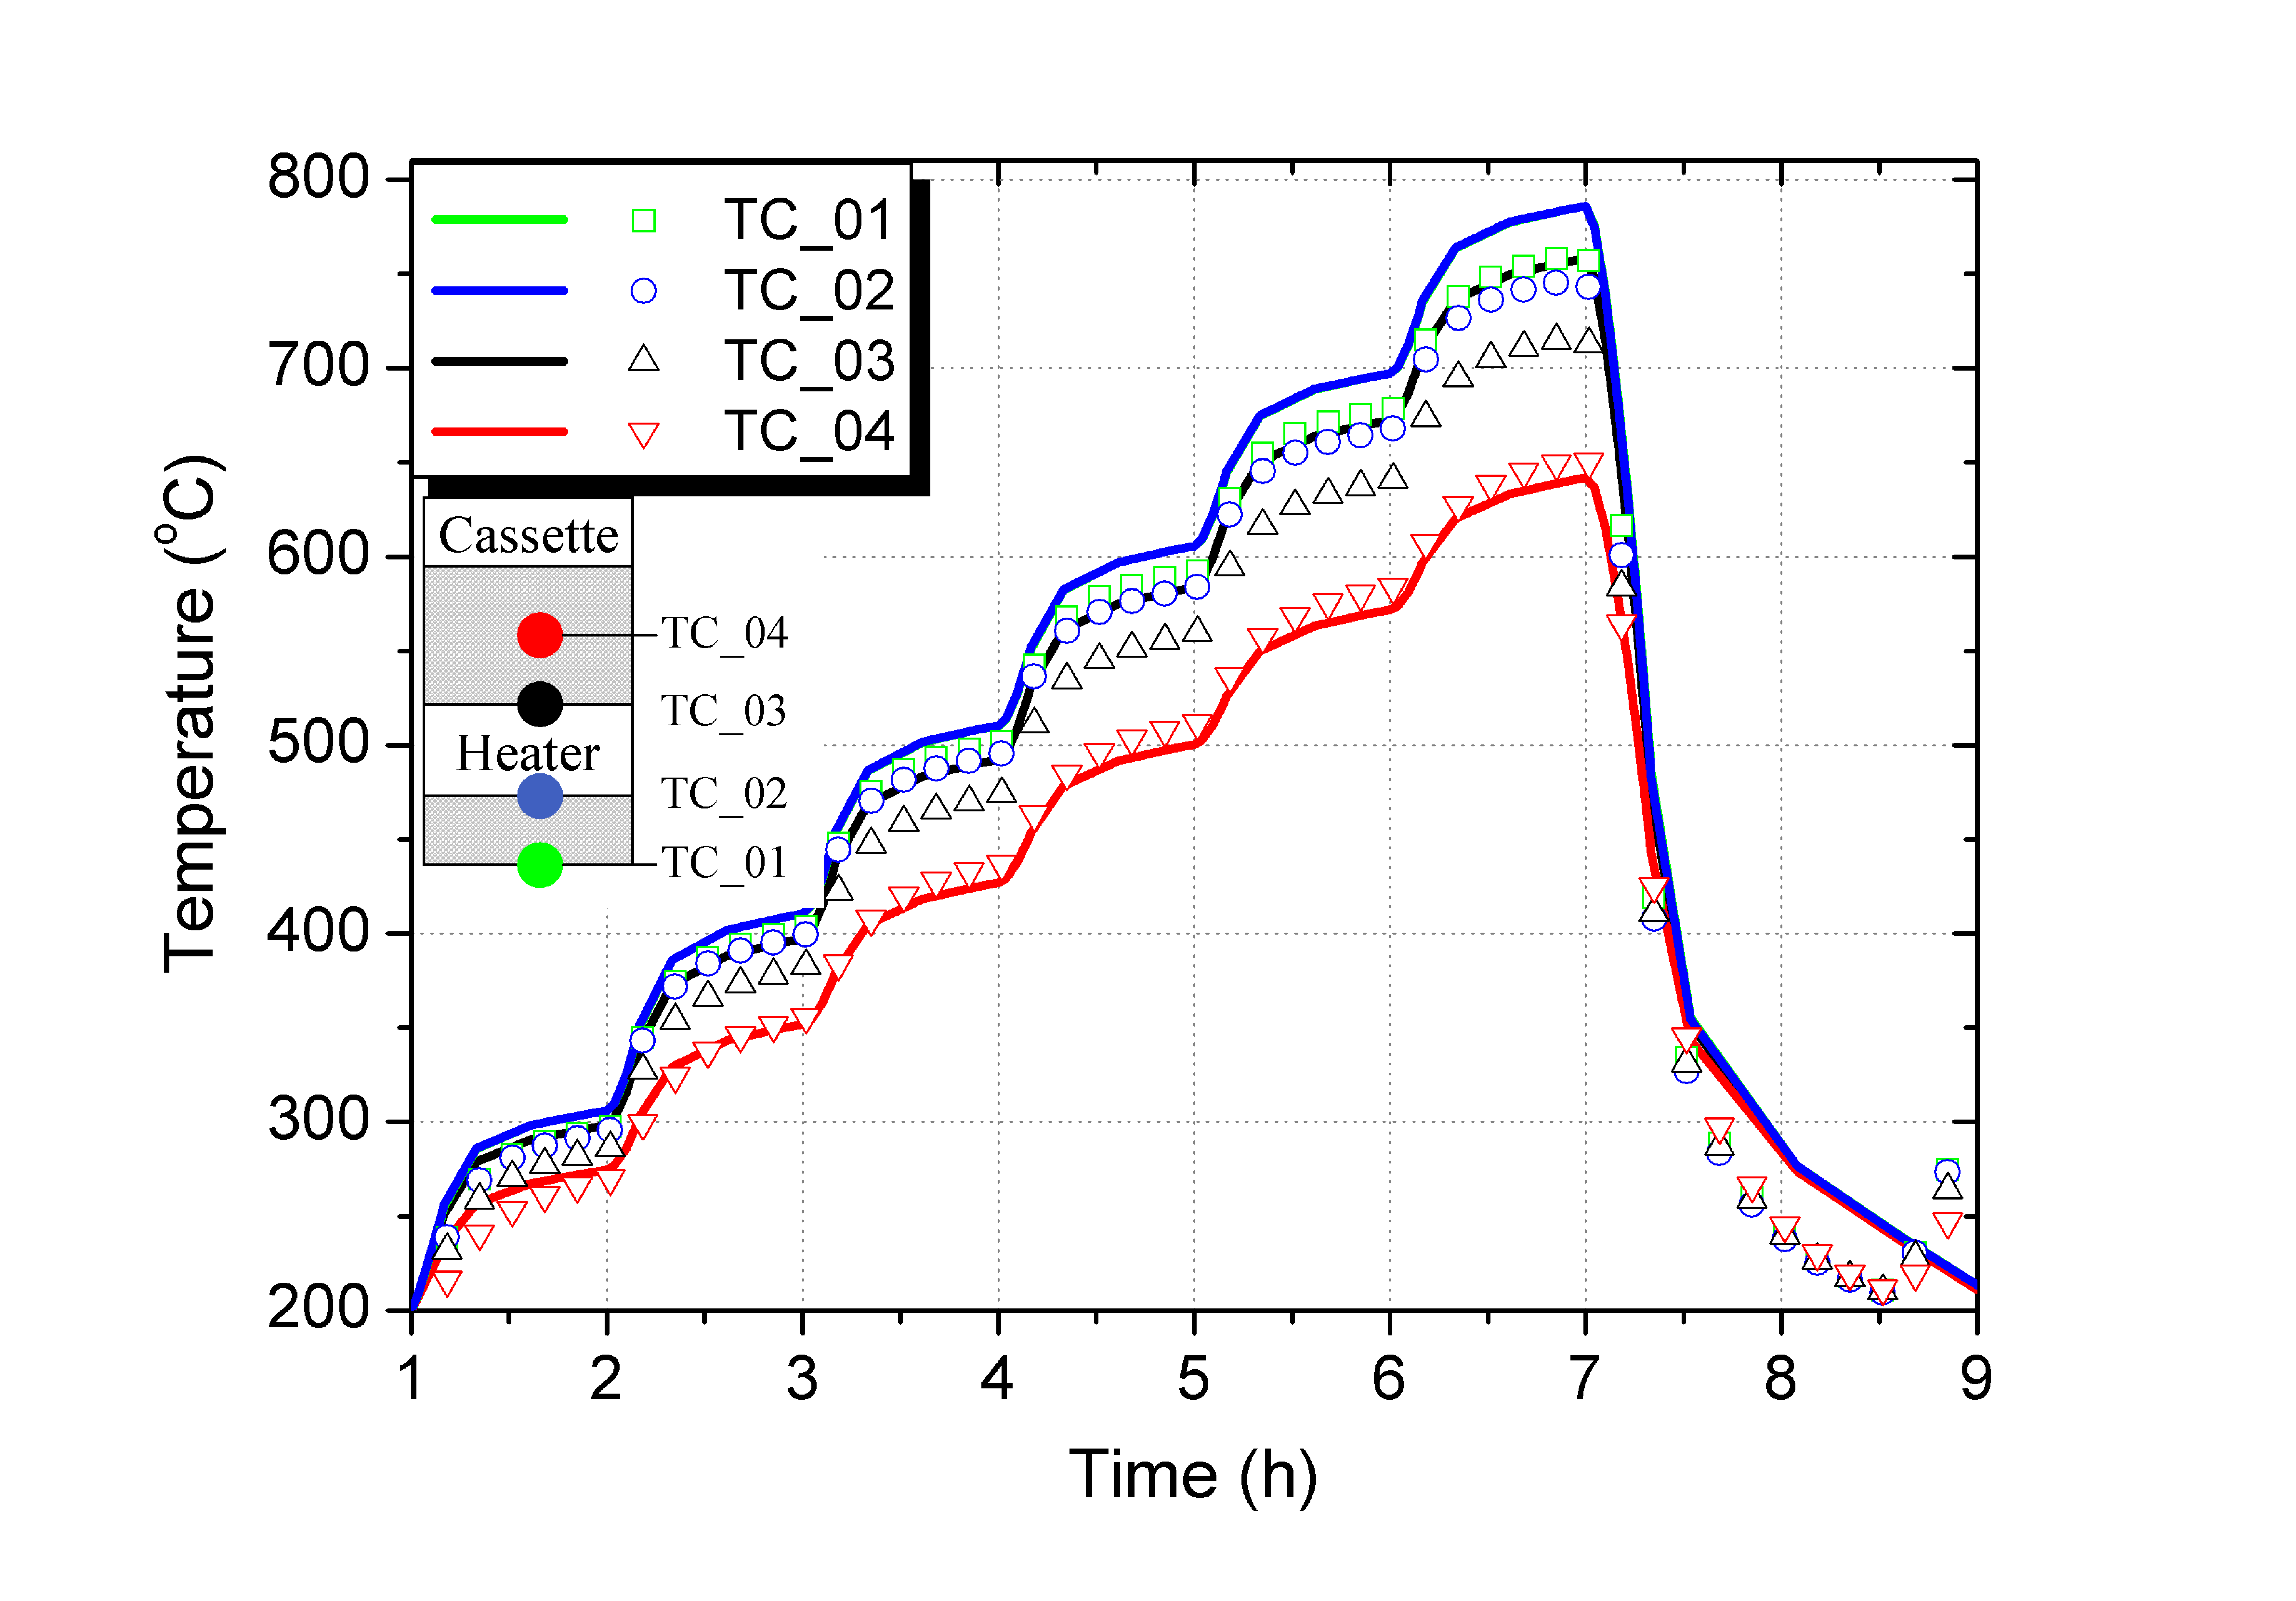
\includegraphics[width=0.5\textwidth]{chapters/figures/Fig-6}
\caption{Results of the FZK benchmarking with HELICA\cite{Gan:2009vn} showing temperature variations with time during a loading cycle (T in $^\circ$C) at 100 mm from FW.}\label{fig:FZK_HELICAa}
\end{figure}

\begin{figure}[t!]
\centering
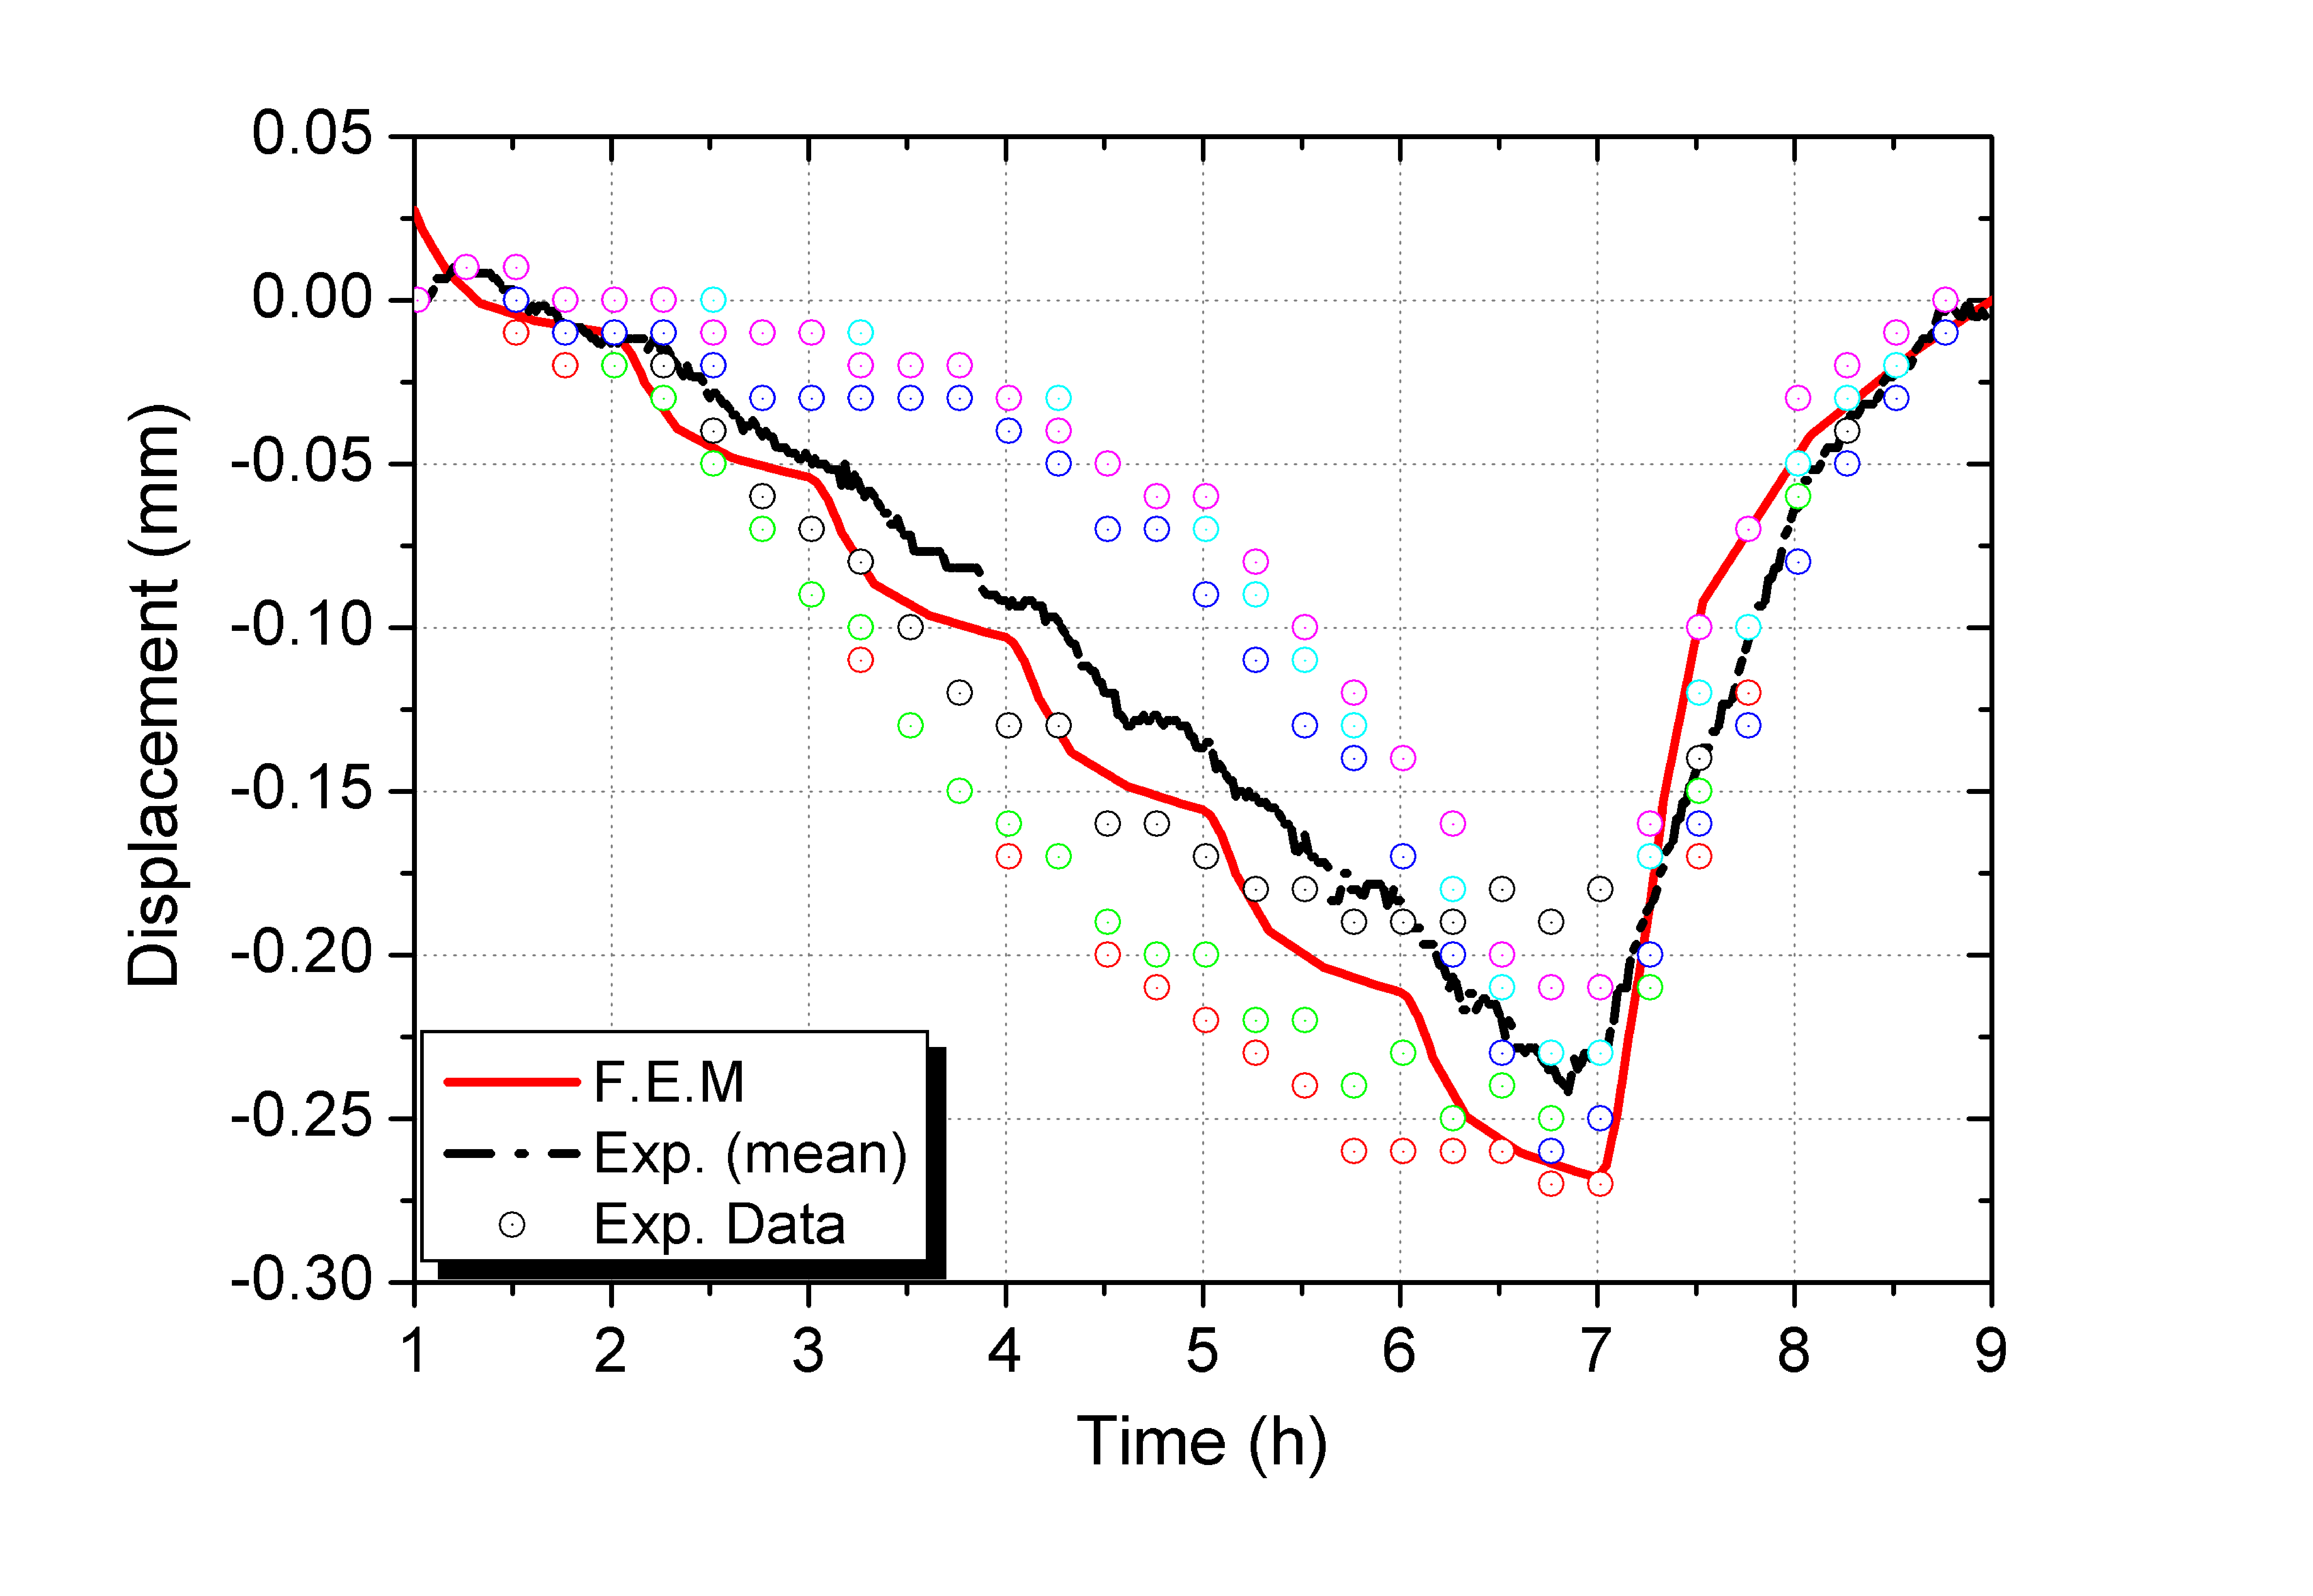
\includegraphics[width=0.5\textwidth]{chapters/figures/Fig-7}
\caption{Results of the FZK benchmarking with HELICA\cite{Gan:2009vn} showing a comparison of displacements (in mm) in HELICA between calculated and measured LVDT values.}
\label{fig:FZK_HELICAb}
\end{figure}

Unfortunately, the ambitions of HEXCALIBER were limited due to the crippling of several heaters. Nevertheless, the limited data was still used in efforts to validate the constitutive relationships of the DIN model. The temperature variations with time were the only major result reported by the ENEA Brasimone team, such as that shown in Fig.~\ref{fig:DIN_HEX}; mechanical results are still forthcoming from the research group. From the comparisons to experimental measurements in HELICA and HEXCALIBER it is encouraging to notice that even in the absence of a creep model, satisfactorily close agreement were seen between computation and measurement. So far, no detailed displacement comparisons have been made to experimental data.

Several important observations are also made from the results of the DIN simulation: (i) three-dimensional effects were important to calculations of the convective energy transport of the helium coolant; future models should continue to be analyzed in three-dimensions; (ii) DIN reports that in HELICA all ceramic beds experience a compressive force everywhere and no gap formation is ever detected. 

In summary, the benchmarking efforts have only recently begun in Europe. A typical pebble bed thermo-mechanics simulation involves first calculating overall temperature fields of the blanket unit as it undergoes volumetric nuclear heating as well as cooling at the boundaries. The non-linear mechanical analysis is then performed for stress and strain estimations. However, since the effective thermal conductivity of the ceramic breeder pebble bed is, to some degree, dependent on strain, a coupled thermal and mechanical analysis is needed. Additional details on modeling steps can be found in Refs.~\cite{DellOrco:2010zr,DiMaio20081287,DiMaio20101234,Gan:2009vn,Gan:2010lh,dellorco:2006}. The two most developed models, from FZK and DIN, have had their results compared to experimental data and have thus far shown great promise. 

However, it must be noted that the benchmarking efforts are incomplete and inconsistencies between the two models must be explained as they move forward. For example, the model of FZK concluded that a gap appeared between the pebble bed and structural wall, however the model from DIN reported no gap formation. The existence of a gap between pebble bed and structural wall will negatively affect the ability to cool the pebble bed and thereby impact structural and tritium release properties of the bed. That such a discrepancy exists between calculated results of the models on such a critical feature warrants either more benchmarking efforts or a careful deconstruction of the constitutive equations to discover the source of the inconsistency. Future experiments aimed at benchmarking ought to focus on creating apparatus capable of expressing, among other things, when gap formation or pebble failure occurs.


\begin{figure}[t!]
\begin{center}
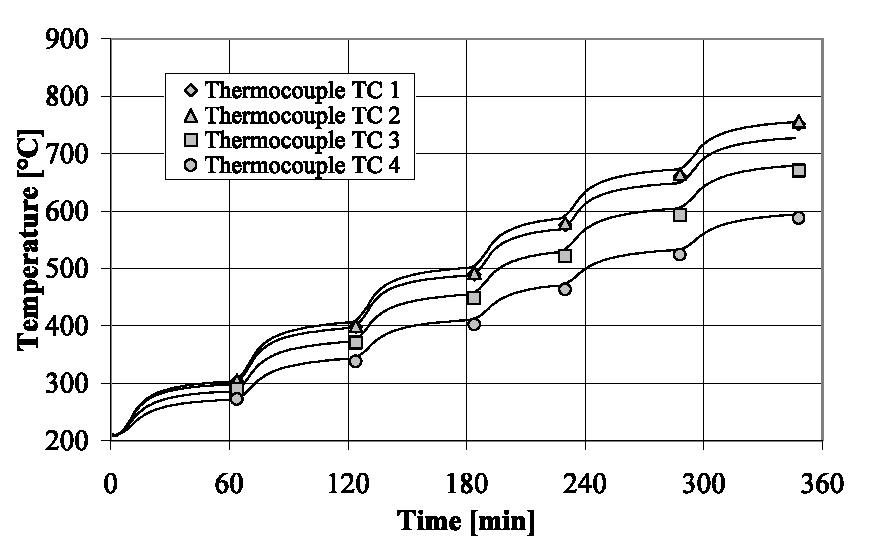
\includegraphics[width=0.4\textwidth]{chapters/figures/Fig-8}
\caption{Exemplary results of the DIN benchmarking with HELICA: Temperature variations with time during a loading cycle at 100 mm from FW\cite{DellOrco:2007hc}.}
\label{fig:DIN_HELICA}
\end{center}
\end{figure}


 \begin{figure}[t!]
\begin{center}
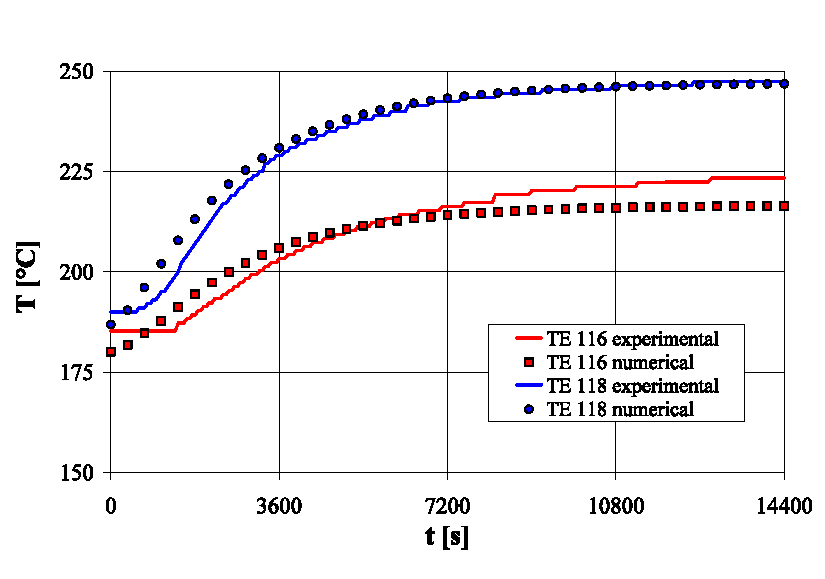
\includegraphics[width=0.4\textwidth]{chapters/figures/Fig-9}
\caption{Exemplary results of the DIN benchmarking with HEXCALIBER : Temperature variations with time during a loading cycle within the first lithium-orthosilicate cell\cite{DellOrco:2010zr}.}
\label{fig:DIN_HEX}
\end{center}
\end{figure}



\subsection{Pebble Bed Assemblies Experiment}
The pebble bed assemblies (PBA) experiment is designed to study the effect of neutron irradiation on the thermo-mechanical behavior of a ceramic breeder pebble-bed under DEMO representative thermo-mechanical loads \cite{Magielsen2007}. This was accomplished via analysis of changes of the in-pile temperature profiles during irradiation as wall as from the post irradiation examination of the pebble bed in the Hot Cells. Within the assemblies, there are four test elements; each resembling a small-scale mock-up of a HCPB TBM with a ceramic breeder pebble bed sandwiched between two beryllium pebble beds. Before irradiation, the beds are pre-compacted with a compressive load of 3 MPa to ensure good settling and contact.  

FEM analysis was performed to study pre-compaction procedures.  During progressive irradiation, temperatures are recorded at several locations in the ceramic breeder bed as well as other critical positions. Reviewing the recorded temperature data, when comparing the temperature in the center of the ceramic breeder pebble bed during later cycles and earlier cycles there appears to be a decrease in temperature for the exact same environmental conditions. Changes in the pebble beds and their characteristics are examined both in-pile by neutron radiography and out-of-pile by e.g. SEM during post-irradiation examination (PIE). The estimated bed height reduction from neutron radiographies over the course of the irradiation has shown 3\% of creep compaction. 

A pebble bed experiencing creep compaction is both becoming more dense as well seeing more-developed inter-pebble conduction paths. The effective thermal conductivity for a creep-compacted ceramic pebble bed is thus expected to be higher than a standard ceramic pebble bed. This phenomenon results in lower temperature gradients and a lower overall temperature magnitude, which is precisely what was observed in the experiment over the course of the cycling. 

During PIE, various microscopy preparation techniques are used to study the deformation state of the pebble beds (signs of creep compaction and sintering), formation of gas gaps between the pebble beds and structural materials, and the interaction layers between eurofer-ceramic and eurofer-beryllium. 

Figure~\ref{fig:pba} shows the cross-section of Li$_2$TiO$_3$ pebbles (left) and Li$_4$SiO$_4$ pebbles (right) post irradiation. Evident in the images is sintering of the lithium titanite and significant fracturing of the lithium orthosilicate pebbles. Importantly, however, it must be noted that the pebble beds performed reliably in spite of the changes displayed in these images cite{magielsen2011}. 


\begin{figure}[t!]
\centering
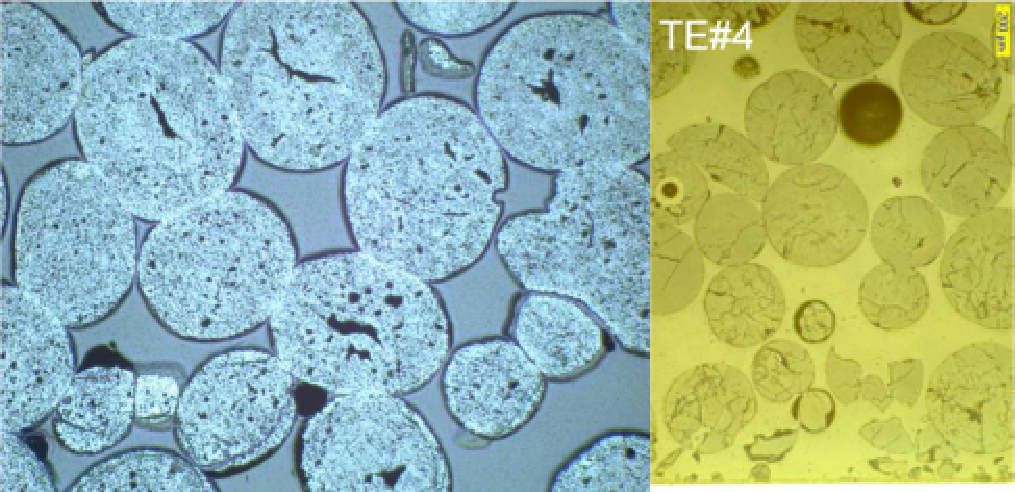
\includegraphics[width=0.5\textwidth]{chapters/figures/Fig-10}
\caption{Notable features of irradiated Li$_2$TiO$_3$ and Li$_4$SiO$_4$ pebble beds from PBAcite{magielsen2011}. (Left) Demonstration of significant sintering of Li$_2$TiO$_3$ pebbles with no fracturing; the visible cracks originated from production and handling. (Right) Demonstration of cracking of Li$_4$SiO$_4$ pebbles.}
\label{fig:pba}
\end{figure}


\subsection{More thermo-mechanics Characterization Experiments}
Coming from the standpoint that strain in a pebble bed is induced by thermal expansion, an experiment was conducted to characterize the pebble bed thermal expansion coefficient \cite{Tanigawa:2007fc}.  The thermal expansion coefficient of a packed \lit pebble bed is measured under a compressive load of 0.1MPa.  The study concludes that for beds with packing factors of 65.3 to 68.5\%, the average thermal expansion coefficient was $(1.4\pm0.2)\times10^{-5}K^{-1}$. This thermal expansion coefficient of the pebble bed was equal to 78\% of that for the bulk material under the conditions used in the study. The reduction in thermal expansion coefficient is less significant than that of the effective modulus, which is more than 2 orders of magnitude smaller than the bulk value. 

The effect of thermal cycling on the packing state is of interest; in particular, it is foreseen that the ITER TBM will be subjected to such conditions. The question that arises is whether a void region will be created under thermal-cyclic loading due to the differential rates of expansion and contraction of the pebble bed and structural containing wall. This uncertainty was first addressed in an experimental set-up involving Li$_2$TiO$_3$ pebbles enclosed by two Kovar flanges while sandwiched between two commercial-grade CVD silicon carbide discs \cite{Calderoni:2006ye}. The set-up allows for generating a high stress through large differential in thermal expansion coefficients. The experimental results indicate that high thermal stresses and deformations are present during the initial thermal cycle of the assembled test article, but are successively alleviated due to a combination of pebble re-arrangement within the bed and creep induced deformation. This suggests that a few thermal cycles under a controlled atmosphere and a compressive load before final assembly of blanket sections would mitigate the severity of the thermal stresses during start-up. This is also shown in a later experiment, in which the increment of compression decreased with each heating cycle and became negligible after 30 cycles \cite{Tanigawa:2010cr}. Extrapolating the finding to a prototypical blanket breeder pebble bed design, the study concludes that for a height of 1 m long pebble bed, a 51 mm high cavity may be generated at the top of the bed with an initial packing of 65\% under thermal cyclic operations.  

\section{Pebble Bed Thermo-mechanics Summary \& Framework}
A good deal of progress has been made in the field of ceramic pebble bed analysis. Owing to the multi-scale nature of pebble beds, it is unavoidable that multi-scale models are necessary. A framework has been envisioned by our group, shown in Fig.~\ref{fig:framework}, the following of which will contribute substantially to the success of the ceramic breeder blanket development. In this framework, the continuum modeling approach using FEM and empirically derived material constitutive equations is capable of correctly characterizing the stress load to which a breeder pebble bed unit may be subject during reactor operation. The DEM approach analyzes this load and determines the possibility of pebble bed morphological changes; i.e. pebble damage based on the crush load data of pebbles, the degree of sintering depending on the local contact stress and temperature fields, and creep relaxation of contacts. It is only with the combined analysis of particle-scale information from DEM and system-scale information from FEM that warrants a high confidence of success to the assembly and design of breeder units in a blanket.  Experiments should also be conducted to assess the manner of pebble relocations and packing rearrangement when morphological evolution of the pebble bed occurs. It is important to learn if the breeder unit will continue to function in accord with the original design goals under all complex operating conditions.  The ultimate objectives of the pebble bed thermo-mechanics are: to delineate a near-equilibrium packing state as the initial state, quantify breeder unit thermo-mechanics parameters during operations, understand how these properties evolve as topographical changes happen in the packing, and ensure breeder functions as it is intended to in the fusion operational phase spaces.

\begin{figure}[t!]
	\begin{center}
	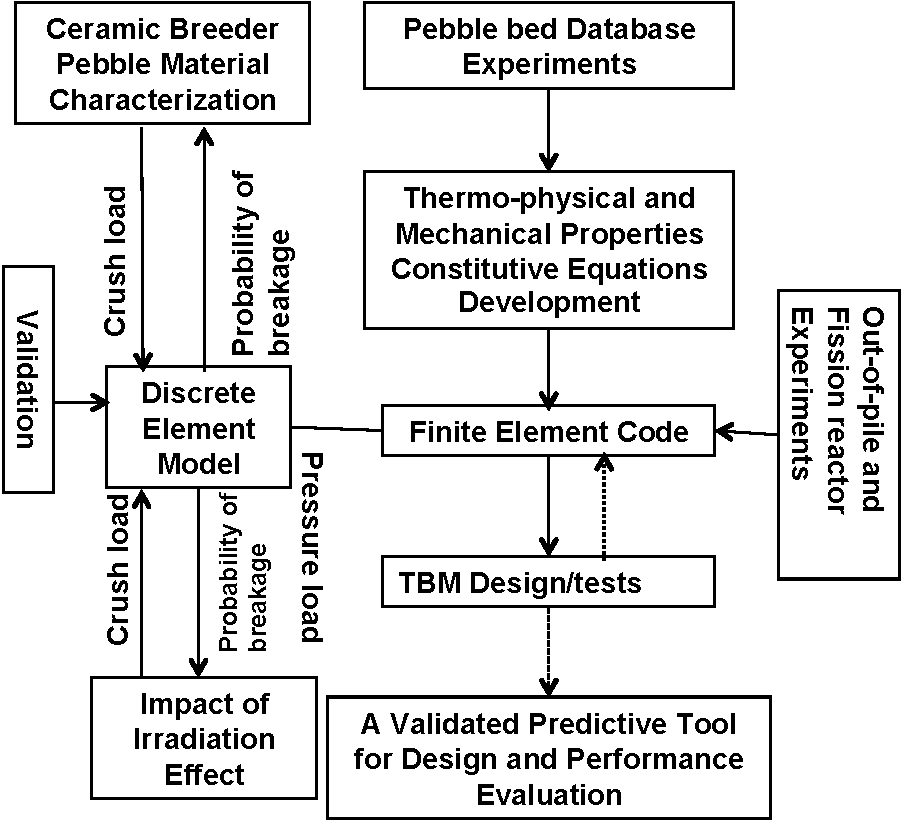
\includegraphics[width=0.5\textwidth]{chapters/figures/Fig-11}
	\caption{Example Pebble Bed Thermo-mechanics Research Framework.}
	\label{fig:framework}
	\end{center}
\end{figure}

Lastly, no predictive tool is possible without solid validation attempts. The benchmark experiments performed up to now were either too limited in scope or practice. New experiments must be performed that can provide reliable data with which to compare numerical results. Fortunately, a new experimental effort out of KIT has been initiated.\cite{Hernandez2014} The experiment shows great promise at reproducing volumetric heating profiles with substantial data collection efforts. The preliminary results are very promising.